
\subsection{Motivating Example}

Sara is a data scientist who is developing an ML model to predict customer churn. Sara begins her project in a Jupyter notebook, which supports iterative development and immediate feedback through the execution of code cells. Her workflow is dynamic and exploratory, typical of modern ML practices. Sara loads the dataset and performs Exploratory Data Analysis (EDA) to develop a high-level understanding of the data she is working with. Since most ML models expect the data to have a normal distribution, Sara generates histograms to validate this assumption. Based on the histograms, Sara confirms that the data has a normal distribution and therefore does not apply any normalisation techniques. With data preprocessing complete, Sara proceeds to build her initial model. After setting up a logistic regression classifier, she runs a training cell that outputs the model's accuracy. The results are disappointing, prompting her to adjust the hyper-parameters of the model in subsequent cells. Each modification is immediately followed by feedback on its impact, allowing Sara to quickly converge on the optimal settings. After all experimentation and model tuning are complete Sara deploys the model into a production environment where the model is periodically retrained using new training data.

% Initially, Sara loads a dataset and uses basic descriptive statistics to understand its distribution. As she executes a cell that calculates and displays the mean and standard deviation of each feature, she notices unusually high variance in one of the features. This insight, derived directly from the output of the notebook cell, prompts her to apply normalisation to ensure better model performance.

A few weeks later, Sara notices a drop in the performance of her model. To investigate, Sara revisits the notebook in which she developed the model. However all the cells in the notebook execute without any errors thus Sara needs to execute each cell individually and manually analyse the outputs which takes considerable amount of time and effort. Sara soon realises that the distribution of the new slice of training data is no longer normal. To fix the issue, Sara applies normalisation techniques. Additionally, she also adds an assertion that performs a K-test 

% sara returns to the notebook since the performance of the model has suddenly dropped. However all cells in the notebook execute without any errors so sara has to execute each cell and analyse the output of the cells manually which takes a long time. Sara finally identifies the source of the problem, the training data is missing 3 features that contributed to the performance of the model. However, sara was unable to identify this since the training data is automatically pulled from a database and another team in sara's organisation changed the db schema without notifying other users

% to ensure that such issues a caught faster in the future, sara adds an assertion that fails if the number of features in the training data changes. This assertion also documents

A few weeks later, Bob is tasked with improving the performance of the model since Sara is on vacation. Bob obtains the notebook in which Sara originally developed the model however is unable to

% Throughout this process, Sara heavily relies on the outputs of various code cells, not just for error correction but also for making strategic decisions about model architecture, such as adding layers or changing activation functions. At one point, after noticing overfitting from a cell outputting validation loss, she decides to incorporate dropout layers, which she can quickly evaluate by rerunning the training process.

% Finally, Sara fine-tunes her model based on the outputs from a confusion matrix and ROC curve, identifying thresholds for classification that balance precision and recall effectively. Each decision in Sara's workflow—--from preprocessing adjustments to hyperparameter tuning and model validation—--is guided by the iterative feedback she receives from the outputs of her notebook's code cells.

% TODO: the jump to assertions is very drastic; motivate it using scenario that there is a bug in the system (use the data validation papers from google) and Sara needs to fix them and how assertions would have helped here to debug the issue faster! (notebook keeps running!)


\subsection{(RQ4) How are assertions used to validate visual outputs in Jupyter notebooks?}~\label{sec:result-rq3}

\subsubsection{Model Performance ($N = 15$)}

\begin{longtable}{@{} m{0.05\textwidth} m{0.4\textwidth} m{0.4\textwidth} @{}}
  \caption{VA pairs used to validate the performance of a model.} \\
  \toprule
  \emph{\textbf{Key}} &
  \emph{\textbf{Visual Output}} &
  \emph{\textbf{Assertion}}\\
  \midrule
  \endfirsthead

  \caption[]{VA pairs used to validate the performance of a model (continued).} \\
  \toprule
  \emph{\textbf{Key}} &
  \emph{\textbf{Visual Output}} &
  \emph{\textbf{Assertion}}\\
  \midrule
  \endhead

  \midrule
  \endfoot

  \bottomrule
  \endlastfoot

  VA2 &
  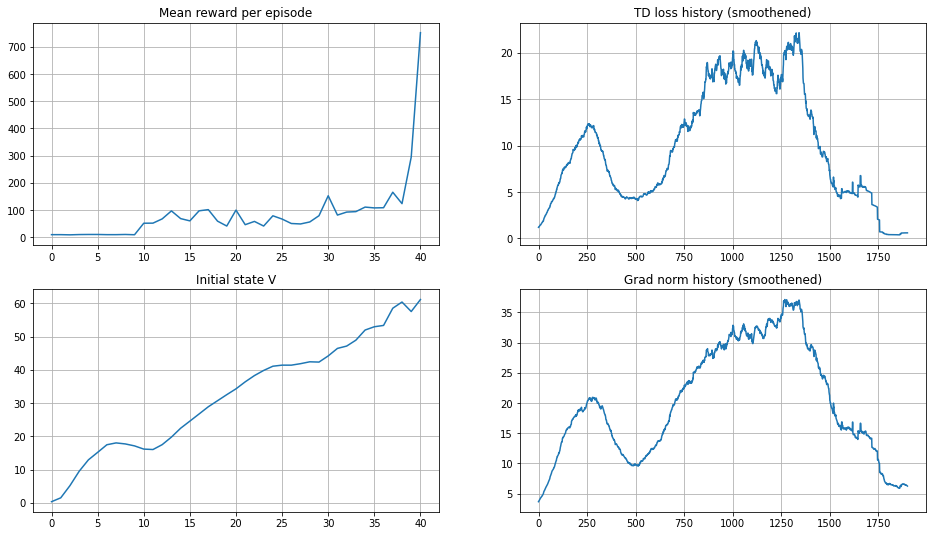
\includegraphics[width=\linewidth]{va2.png} &
  \lstinline[]$assert final_score > 300, 'not good enough for DQN'$\\

  VA3 &
  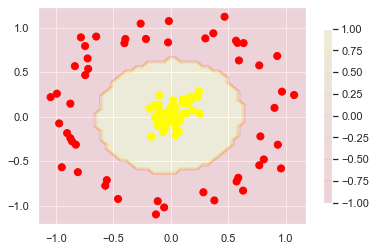
\includegraphics[width=\linewidth]{va3.png} &
  \lstinline[]$assert accuracy_score(y_test, pred) > 0.95$\\

  VA9 &
  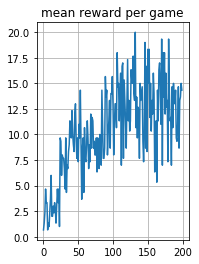
\includegraphics[width=\linewidth]{va9.png} &
  \lstinline[]$assert np.mean(mean_rw_history[-10:]) > 10.$\\

  VA11 &
  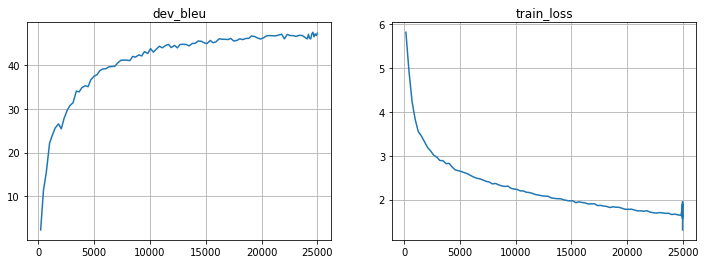
\includegraphics[width=\linewidth]{va11.png} &
  \lstinline[]$assert np.mean(metrics['dev_bleu'][-10:], axis=0)[1] > 35, "We kind of need a higher bleu BLEU from you. Kind of right now."$\\

  VA15 &
  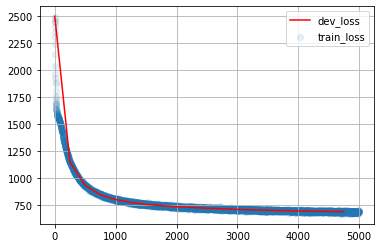
\includegraphics[width=\linewidth]{va15.png} &
  \lstinline[]$assert np.mean(train_history[:10], axis=0)[1] > np.mean(train_history[-10:], axis=0)[1], "The model didn't converge."$\\

  VA28 &
  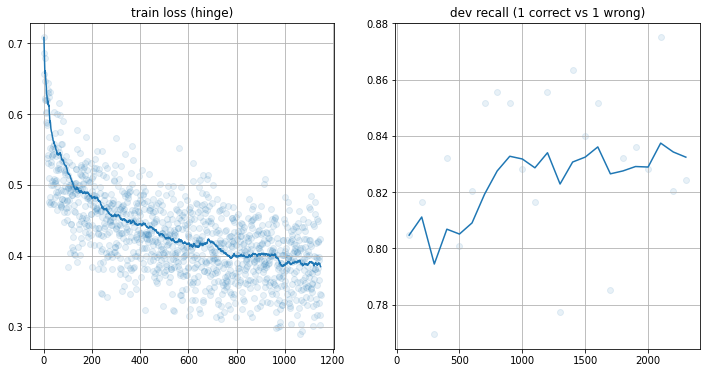
\includegraphics[width=\linewidth]{va28.png} &
  \lstinline[]$assert np.mean(dev_recall_history[-10:]) > 0.85, "Please train for at least 85% recall on test set. You may need to change vectorizer model for that."$\\

  VA68 &
  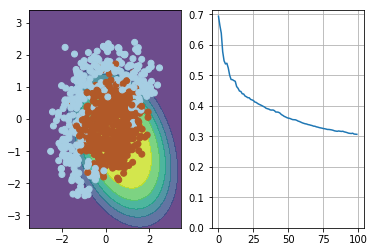
\includegraphics[width=\linewidth]{va68.png} &
  \lstinline[]$np.testing.assert_almost_equal(ans4, 0.3042764)$\\

  VA107 &
  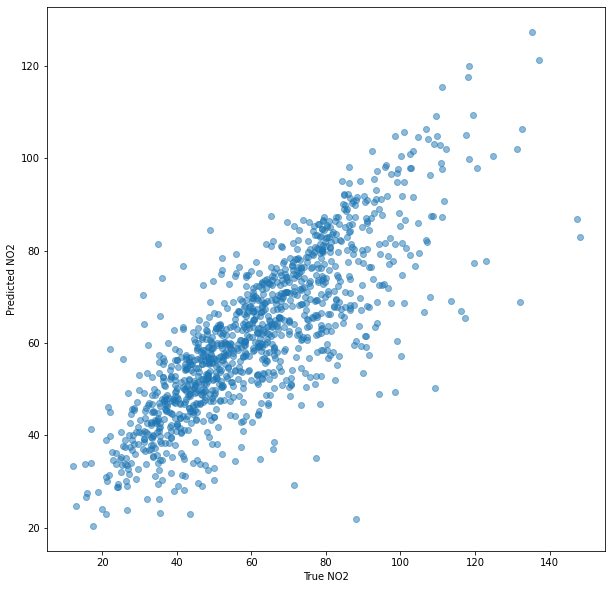
\includegraphics[width=\linewidth]{va107.png} &
  \lstinline[]$assert r2_gru > 0.6$\\

\end{longtable}\label{tab:va-model-perf}

The visualisations in VA2, VA9, and VA15 provide a comprehensive view of key metrics for evaluating the performance of various machine learning models. VA2 includes mean reward per episode, TD loss history, initial state value (V), and gradient norm history for a Deep Q-Network (DQN) model. These metrics collectively indicate the model's learning progress and stability during training. The visualisation in VA9 shows the mean reward per game for a DQN applied to the Breakout Atari game, tracking the model's performance over 200 games. The general upward trend indicates learning and improvement in gameplay over time. VA15 presents the training and development loss over time for a character-level language model, showing a gradual decrease in loss and suggesting effective learning.

The visualisation in VA3 presents a two-dimensional scatter plot showing the decision boundary of a Support Vector Machine (SVM) model, with red and yellow points representing two different classes and a background colour gradient indicating the decision function of the SVM. This visualisation aids in understanding the model's ability to distinguish between classes and the distance of the samples from the decision boundary. The visualisations in VA28 display the training loss and development recall, respectively. The left graph shows a decrease in training loss over time, indicating learning progress, while the right graph shows development recall over time, highlighting improvements in the model's ability to correctly identify positive instances. The visualisations in VA11 depict key metrics for evaluating the performance of a machine learning model in text generation or machine translation. The left plot shows a steady increase in the development BLEU score over the training iterations, indicating improving quality of the model's output, while the right plot displays a steady decrease in training loss, suggesting effective learning and error minimization. In VA107, the scatter plot displays the predicted versus true values of Nitrogen Dioxide (NO2) levels, used to assess the model's performance in predicting continuous variables.

The corresponding assertions for these visualisations ensure that the models meet specific performance standards. For VA2, the assertion ensures that the final score exceeds 300, validating the model's performance for deployment. In VA9, the assertion checks whether the mean of the last ten rewards exceeds 10, ensuring stable and satisfactory learning progress. For VA15, the assertion checks if the mean of the first ten training observations is greater than the mean of the last ten, ensuring loss convergence and validating the model's learning without overfitting. The assertion in VA3 ensures the accuracy score on the test set exceeds 0.95, confirming the model's reliability and generalization capability. For VA28, the assertion checks whether the average development recall in the last ten evaluations exceeds 0.85, ensuring high recall rate critical for tasks like medical diagnostics. In VA11, the assertion ensures the average development BLEU score in the last ten evaluations exceeds 35, confirming the model produces high-quality translations. Lastly, in VA107, the assertion checks whether the R2 score exceeds 0.6, validating the model's fit and reliability for making accurate predictions in real-world scenarios. These validations confirm that iterative training processes lead to meaningful improvements and ensure the models' readiness for deployment and practical applications.

\highlight{\textbf{Finding 3.1} 15 VA pairs are used to evaluate the performance of ML models. The visualisations include metrics such as mean reward, training loss, accuracy, BLEU scores, and R2 scores. Assertions associated with these visualisations ensure models meet a specific performance criteria.}

\subsubsection{Distribution Check ($N = 1$)}

\begin{table}
  \centering
  \caption{VA pairs used to check data distribution.}
  \begin{tabular}{@{} m{0.05\textwidth} m{0.4\textwidth} m{0.4\textwidth} @{}}
    \toprule
    \emph{\textbf{Key}}&
    \emph{\textbf{Visual Output}}&
    \emph{\textbf{Assertion}}\\
    \midrule

    VA13 &
    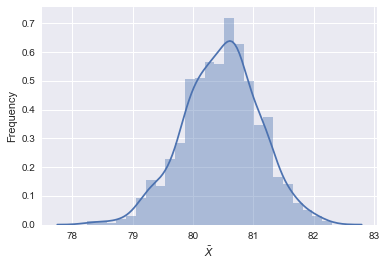
\includegraphics[width=\linewidth]{va13.png} &
    \lstinline[]$assert 80 < boot_mean_mean < 81$\\
    \bottomrule
  \end{tabular}
  \label{tab:va-dist-check}
\end{table}

The visualisation in VA13 displays the distribution of bootstrapped sample means as a histogram with a superimposed kernel density estimate (KDE) curve, illustrating the central tendency and variability of the bootstrapped means.

Bootstrapped sample means are calculated by repeatedly resampling the original dataset with replacement and computing the mean for each resampled dataset. This process generates a distribution of the mean, known as the bootstrap distribution, which helps in estimating the variability and central tendency of the original dataset's mean.

The corresponding assertion checks whether the bootstrapped mean lies between 80 and 81, ensuring that the statistical estimation is consistent with expected values. This validation is crucial for confirming the reliability of the bootstrapped estimates and the accuracy of statistical conclusions.

\highlight{\textbf{Finding 3.1} One visualisation is used to display the distribution of bootstrapped sample means. The corresponding assertion checks if the bootstrapped mean lies between a specific range, ensuring a consistent statistical estimation.}

\subsubsection{Data Validation ($N = 9$)}

\begin{longtable}{@{} m{0.05\textwidth} m{0.4\textwidth} m{0.4\textwidth} @{}}
  \caption{VA pairs used for data validation.} \\
  \toprule
  \emph{\textbf{Key}} &
  \emph{\textbf{Visual Output}} &
  \emph{\textbf{Assertion}}\\
  \midrule
  \endfirsthead

  \caption[]{VA pairs used for data validation (continued).} \\
  \toprule
  \emph{\textbf{Key}} &
  \emph{\textbf{Visual Output}} &
  \emph{\textbf{Assertion}}\\
  \midrule
  \endhead

  \midrule
  \endfoot

  \bottomrule
  \endlastfoot

  VA30 &
  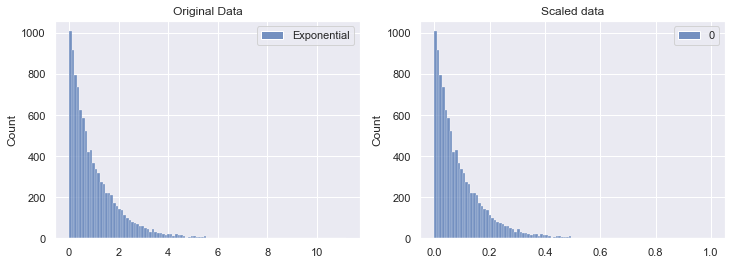
\includegraphics[width=\linewidth]{va30.png} &
  \lstinline[]$assert scaled_data[scaled_data.argmax()] <= 1$\\

  V35 &
  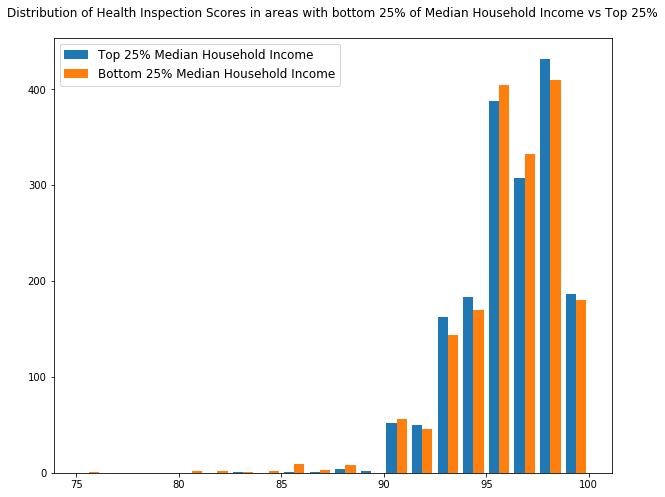
\includegraphics[width=\linewidth]{va35.png} &
  \lstinline[]$assert(all(df_lower['inspection_score'] > 75))$\\

  V57 &
  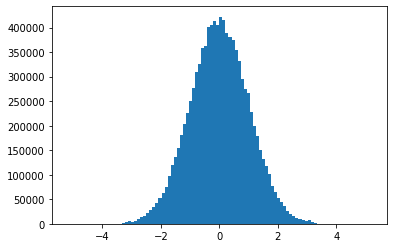
\includegraphics[width=\linewidth]{va57.png} &
  \lstinline[]$assert kstest(data_transformed[:, feature], 'norm').statistic < 1e-2$\\

  VA62 &
  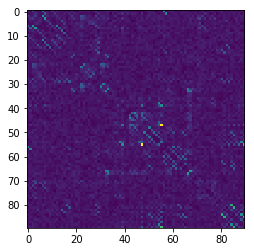
\includegraphics[width=\linewidth]{va62.png} &
  \lstinline[]$assert not np.allclose(x_aug, x_original)$\\

\end{longtable}\label{tab:va-data-validatio}

The VA pairs in Table~\ref{tab:va-data-validatio} collectively illustrate various data validation techniques essential for ensuring the integrity and quality of data used in ML models. 

The visualisation in VA30 consists of two histograms comparing the original and scaled distributions of an exponential dataset. The left plot shows the distribution of the original data, while the right plot displays the distribution after scaling. The scaling process adjusts the data to fall within a specified range of 0 and 1. The corresponding assertion checks whether the maximum value in the scaled data is less than or equal to 1, ensuring that the scaling procedure was applied correctly.

The visualisation in VA35 shows the distribution of health inspection scores in areas with the bottom 25\% and top 25\% of median household income. The blue bars represent areas with the top 25\% median household income, while the orange bars represent areas with the bottom 25\%. This comparison helps identify any disparities in health inspection scores based on income levels. The corresponding assertion checks that all inspection scores in the lower-income areas are above 75, ensuring that the data reflects a minimum standard of health inspection scores in these areas.

The visualisation in VA57 shows a histogram of transformed data after it has been normalised. The corresponding assertion checks that the Kolmogorov-Smirnov (KS) test statistic for the transformed data is less than $1 \times 10^{-2}$, ensuring that the data closely follows a normal distribution.

The visualisation in VA62 displays a heatmap of an augmented dataset generated using a weighted k-nearest-neighbors (k-NN) method. This heatmap helps in visualizing the differences and similarities between the original and augmented data. The corresponding assertion checks that the augmented data \lstinline{x_aug} is not nearly identical to the original data \lstinline{x_original}, ensuring that the data augmentation process has introduced sufficient variability.

These validations are crucial for confirming that data preprocessing techniques such as scaling, transformation, and augmentation have been correctly applied. Ensuring the integrity and quality of the data is essential for the subsequent steps in the machine learning pipeline, as it directly impacts the robustness, reliability, and generalization of the models developed. By validating these steps, we can maintain high standards of data quality and model performance, which are fundamental for accurate and meaningful analyses.

\highlight{\textbf{Finding 3.3} Nine VA pairs focus on data validation tasks such as comparing the original with the scaled data distribution and ensuring augmented data is different from the original. These validations confirm that data preprocessing steps like scaling, transformation, and augmentation are correctly applied.}

